%%%%%%%%%%%%%%%%%%%%%%%%%%%%%%%%%%%%%%%%%%%%%%%%%%%%%%%%%%%%%%%%%%%%%%%%%%%
%%%%%%%%%%%%%%%%%%%%%%%%%%%%%%%%%%%%%%%%%%%%%%%%%%%%%%%%%%%%%%%%%%%%%%%%%%%
\section{Design Principles of Recoil Separators}
% Experimental requirements, theory of separators, figures of merit
\label{design}

In this section we will present the equations for the motion of charged particles in magnetic and electric fields before discussing the types and design of ion-optical elements required in different designs of recoil separators, as well as exploring some of the rigidity and performance regimes for astrophysically important radiative capture reactions. In addition we discuss the various types of gas targets that can be used with a recoil separator.

%%%%%%%%%%%%%%%%%%%%%%%%%%%%%%%%%%%%%%%%%%%%%%%%%%%%%%%%%%%%%%%%%%%%%%%%%%%
\subsection{Ion Optical Elements}
\label{ion}

For a recoil separator to function, it in principle has to induce a spacial separation between unreacted beam and recoil particles of different mass but similar momentum. In addition, it has to accept recoils with finite angles with respect to the beam axis. In almost all cases discussed in this paper polarized beams are not used, therefore recoils are uniformly distributed in azimuthal angle, $\phi$. 
Thus in order for recoils to be separated, they must be brought to a focus in a mass-dispersed plane at some point. Due to the typical rigidities experienced in inverse kinematics at astrophysically-relevant energies, magnetic elements are required to provide the focusing. Electrostatic elements or combined electrostatic and magnetic elements are used in addition to these to provide mass dispersion or beam rejection.  

The motion of a charged particle (with charge $q$) in external electromagnetic fields $\vec{\mathcal{E}}$ and $\vec{B}$  is governed (non-relativistically) by the Lorentz force equation:

\begin{equation}
\vec{F}=\frac{d\vec{p}}{dt}=q(\vec{\mathcal{E}}+\vec{v}\times\vec{B})
\end{equation}   

where $\vec{v}$ is the instantaneous particle velocity. 

In addition, we can define the charged particle {\em rigidity}, which is a measure of how difficult it is to bend the particle trajectory in a uniform electric or magnetic field. The magnetic rigidity, derived by considering the circular motion of the particle in a purely magnetic field of constant magnitude, is given by

\begin{equation}
\label{magrigidity}
\mathcal{R}_\mathrm{M}=|\vec{B}|\rho=\frac{p}{q}
\end{equation}

where $|\vec{B}|$ is the field magnitude, $\rho$ is the radius of the circular trajectory taken by the charged particle, $p$ is the particle momentum (assumed perpendicular to the field direction), and $q$ is the charge.

The electric rigidity, derived by considering the circular motion of the particle in a purely electric field of constant magnitude, is given by

\begin{equation}
\mathcal{R}_\mathrm{E}=|\vec{\mathcal{E}}|\rho=\frac{pv}{q}
\end{equation}

where $|\vec{\mathcal{E}}|$ is the field magnitude, $\rho$ is the radius of the circular trajectory taken by the charged particle, $p$ is the particle momentum (assumed perpendicular to the field direction), $v$ is the particle velocity, and $q$ is the charge.


%%%%%
\subsubsection{Magnetic elements -- focussing and momentum/charge dispersion}\label{magel}

%\small
%\begin{itemize}
%\item What are the necessary equations to present?
%\item path of a charged particle in a magnetic field
%\item image/object relationship
%\item typical field strengths
%\item double focussing, sextupole correction
%\item its function as a momentum filter in our application means that we use it as a charge state filter because beam and reaction recoil have very similar central momentum
%\item give equation for position of charge states blocked by slits
%\end{itemize}
%\normalsize

Magnetic quadrupoles are required in order to produce foci for the transported ions in the separator. This is usually achieved via doublets or triplets, providing net focussing in both the horizontal and vertical planes. While doublets are suitable for the bulk of the focussing\footnote{Note that an antisymmetric doublet, one whose field gradients and effective lengths are equal, cannot provide a true stigmatic focus, instead transforming a circular source image into an ellipse. With a general doublet however stigmatic operation is possible \cite{reg67}.}, triplets may be required prior to a focus with more stringent requirements. This is due to the fact that in doublets changes in field strength in one focussing plane might introduce undesirable changes in the other plane. Triplets offer an extra degree of freedom to work with in obtaining the focal properties of interest.  

Quadrupoles have focal lengths that are rigidity- and effective-length-, and field-gradient-dependent, and thus must have the applied field scaled according to the ion charge, mass and energy.  With typical effective lengths of quadrupole magnets usually on the order of 0.2-0.5 metres for the momenta under consideration here, the strengths required for effective focussing will depend on the field gradient required and thus the quadrupole bore, but for most recoil separator applications, field strengths are on the order of 0.1 Tesla at the pole tip. Due to the difficulty of achieving perfect focussing properties using simple quadrupole doublets and triplets, higher order multipole magnets are sometimes used to make corrections for aberrations induced by the quadrupoles. Primarily, separate sextupole magnets can be combined with the doublets and triplets. These correct for the typical spherical and `coma'-type aberrations. In addition, quadrupole magnets can be constructed with pole-tip shaping that induces a sextupole or higher-order component.  

Beam-target and recoil-target interactions will result in a distribution of ion charge-states being propagated through the separator. In order to bring the ions to a unique mass-dispersed focus there must be some form of momentum and charge filter. The least complex way to do this would be the use of a magnetic dipole field in combination with quadrupole focussing. A magnetic dipole placed after a stigmatic doublet would provide dispersion in momentum for a given charge (or dispersion in charge for a given momentum). \\
Simplistically (neglecting fringe fields), from equation \ref{magrigidity} it can be seen that since the momenta of recoil ions will typically vary only within $\pm2\%$ or so of the beam momentum value, such a device cannot be used as a mass separator, with bending angles being very close to each other for a given charge state. However since neighbouring charge states are usually different by a large fraction of the charge state value, bending angle differences are larger. This means spacial separation of neighbouring charge states can be significant in the focal plane, and slits can be used to reject the unwanted components. One can say to a good approximation that $\Delta \rho / \rho \approx \Delta q / q$. In addition, a low energy tail in the beam/recoils, perhaps induced by electrostatic elements in the accelerator or even small angle scattering within the separator target region, can be rejected after this device. In practice, magnetic dipoles will have shaped pole edges that mitigate field-gradient issues and lead to improved focussing.

%%%%%
\subsubsection{Electrostatic elements}

%\small
%\begin{itemize}
%\item path of a charged particle in an electrostatic field
%\item typical necessary field strength/curvature for our application
%\item focussing issues
%\item acts as an energy filter
%\item where does the not transmitted beam/charge states end up (split electrode approach, gridded possibility?)
%\end{itemize}
%\normalsize

A cathode and anode in the form of segments of concentric cylinders can produce a radial electric field which has constant magnitude $\mathcal{E}$  at a given radius between the cylinders.   Ions having a suitable electric rigidity can travel at a constant radius through the device. Such an electrostatic dipole will deflect reaction products and beam ions through different angles due to their different velocities, resulting in differing $x$ positions in the focal plane given by $x-x_0\approx\frac{p(v-v_0)}{q\mathcal{E}}$. Such separation, as a fraction of the bending radius, will be on the order of the fractional beam-recoil mass difference, which will usually, for most cases considered in past astrophysical recoil separators, be larger than the spread in recoil momenta. Thus at such a mass-dispersed focus, slits can be placed to provide beam rejection while allowing the recoil ions to pass through.   However, a low-energy tail of the beam, in a lower charge state and having the same electric rigidity as the reaction product, will not be separated. This short-coming can be remedied by combining a magnetic dipole and electrostatic dipole in such a way that a subsequent angular focus is also a focus in ion energy (achromatic) but is dispersed according to ion mass.  

The required electrostatic fields are of order megavolts per metre.  Extensive measures, such as polishing the electrodes to a mirror finish, are required to prevent voltage breakdowns.   Because an electrostatic dipole must deflect desired particles through a permanently-fixed angle,  an experiment  cannot be performed unless the requisite   electrode voltages can be achieved. A CW multiplier stack can be used to achieve the high voltages on the electrodes. The usual design of such a device consists of a steel vacuum tank containing the electrodes, and two cylindrical stack regions containing the multiplier and filled  with an inert insulating gas such as SF$_{6}$, though devices with external high-voltage supplies can be used depending on the separator layout geometry. The devices are prone to electrical breakdown, either in the region between the electrodes or in other high-field regions. This can be due to impurities on the HV surfaces or other non-uniformities like small protrusions of electrode metal that can form. In each case breakdown results in the generation of x-rays with a spectrum dependent on the applied voltage. Therefore a significant amount of shielding is required on the device to protect users from radiation fields during any conditioning phase of the electrodes. In addition, field electron emission becomes important in the consideration of maintaining significantly high voltages on these devices, and in the ambient x-ray flux produced and possible breakdown \cite{Dia98a}. The phenomenon of gas desorption is also to be considered as a source of electrical breakdown \cite{Dia98b}, and in part motivates the need for high vacuum at the $<10^{-7}$ mbar level between HV gaps. 
\\
One method of conditioning of these devices consists of slowly stepping up the voltage allowing the generation of sparks that will produce an allowable flux of x-rays, stepping back down in voltage when the flux climbs above a predetermined threshold. These sparks will burn off the impurities that cause them, allowing an overall voltage increase. Once operational voltage is achieved the ambient x-ray flux should be negligible and in principle the electrodes hold their conditioning under vacuum indefinitely at high voltage, self-regulating any impurities. Readback current in the power supplies can also be used as a conditioning diagnostic. Long periods at lower voltage can cause the conditioning to be lost, as can a drastic change in vacuum properties. In the case of protrusion impurities inert, moderately heavy, gas such as argon can be introduced to the system during conditioning, the idea being that ions are made during sparks that can provide enough energy to etch away the whisker. As will be seen in later sections, such devices have successfully achieved electric fields of up to 4.6 MV/m.  

%%%%%
\subsubsection{Combined crossed field (Wien) filter elements}

%\small
%\begin{itemize}
%\item what conditions have to be met to transmit the recoils (E,B field selection, condition)
%\item what is the equation which tells us where the not transmitted beam and other charge states end up
%\item typical fields and dimensions for our application
%\end{itemize}
%\normalsize

In a Wien filter parallel flat electrodes between the poles of a magnet provide crossed electric and magnetic fields, $\mathcal{E}$ and $B$.      There is a certain ratio $\mathcal{E}/B$ which results in ions of velocity $v$  undergoing no deflection as they pass through the Wien filter, regardless of their momentum $p$ or charge $q$.    Accordingly, a Wien filter can be tuned to pass the desired reaction product straight through while deflecting beam ions.  Like the electrostatic dipole, it may pass beam particles in  a low-energy tail; unlike the electrostatic dipole, it  also allows   neutral particles to pass through.

Because it is  the ratio $\mathcal{E}/B$ which selects the velocity, a Wien filter may operate with reduced\ field strengths (and reduced mass resolving power)  in order to accommodate reaction products of high rigidity, or if there is a problem reaching the designed maximum electric field.    On the other hand, a Wien filter poses greater design problems, requiring careful shaping of both the electrodes and the magnet poles in order to achieve the desired field uniformities and to match fringe fields. 

In general a Wien filter suffers from the same high voltage conditioning constraints as electrostatic dipole devices,. In addition, some Wien filters use external high voltage supplies, such as in some muon spin rotator systems (e.g. M20 facility, TRIUMF \cite{bev85}). 

%%%%%%%%%%%%%%%%%%%%%%%%%%%%%%%%%%%%%%%%%%%%%%%%%%%%%%%%%%%%%%%%%%%%%%%%%%%
\subsection{Performance}
\label{performance}

%%%%%
\subsubsection{Beam suppression}
Reaction yield and detector performance together define the requirements for beam suppression by the separator.    The most challenging reactions  may well call for suppression by 10 to 12 orders of magnitude.    Separator designs for fusion-evaporation reactions, with higher yields and larger beam-product mass differences, may not be the best models  for radiative capture experiments.   
    
 One class of potential background is the tail of a  distribution generated by many small interactions, such as multiple scattering or energy straggling in the target.    Typically, these distributions have a Gaussian shape near their maximum but after only a few  ``standard deviations" the distributions become dominated by single large-deviation interactions, such as nuclear scattering in the target.    More complicated to assess are single scatterings from residual gas somewhere within the separator.   Nevertheless, it may be possible to investigate by computer simulation whether  a proposed separator design is able to suppress such events.
 
  ``Black Swan" events pose the most difficult problem for the separator designer.   By definition extremely rare and hard to foresee,  they are not  amenable to realistic simulation by computer.   Typically, they may involve sequential scatterings from  solid surfaces inside the separator.   The ranges of beam ions in solids being on order 1--100~$\mu$m, the surface material and roughness at the micrometer scale play a big role: oblique incidence on a smooth surface should be avoided and if possible such surfaces should be masked.   The separator designer must look to defence in depth, with more beam suppression features than the minimum required for events of the first  class.

%%%%%
  \subsubsection{Figure of merit}
  Some specifications, taken in combination, impose minimum requirements on the strength and extent of electric and magnetic fields.   These are the mass resolving power ($P_\mathrm{m}$), the angular acceptance ($\Delta a$) and the particle rigidity 
  ($\mathcal{R}_\mathrm{M}=p/q$ or $\mathcal{R}_\mathrm{E}=pv/q$).    
  Consider a source of ions (reactions in the target), a dispersive device  (radius of curvature $\rho$) and an image (focal) plane.   The  trajectories of the ions having the extremes in initial angles will delimit an area ($A$)  in the bend-plane of the dispersive device.     The first order resolving power is given by the linear magnification ($M$) of the image, the mass dispersion ($D$) and the transverse source size ($\Delta x$): 
  $P_\mathrm{m} = D/(M \cdot \Delta x) $. 
  It has long been known (see, for example, \cite{Wo71}) that source emittance and the resolving power can be related to properties of the dispersive device by
  \[ P_\mathrm{m}\  \Delta a\  \Delta x = A/\rho \]
  Recalling that 
  $\mathcal{R}_\mathrm{M}=\rho \ B$ and $\mathcal{R}_\mathrm{E}=\rho \ \mathcal{E}$,  we obtain  figures of merit 
  \[ P_\mathrm{m}\  \Delta a\  \Delta x \ \mathcal{R}_\mathrm{M} = A \cdot B \]
   \[P_\mathrm{m}\  \Delta a\  \Delta x \ \mathcal{R}_\mathrm{E} = A \cdot \mathcal{E} \]
   That is, to achieve a certain figure of merit it is necessary to have a certain minimum product of field strength and area.  For an electrostatic device it may be convenient to use the length of electrodes and the gap between them as a proxy for the area $A$.  Then, the figure of merit becomes $L\cdot\Delta V$, where $L$ is the length of the electrodes and $\Delta V$ is the voltage difference between them.
   
%%%%%
\subsubsection{Charge changing cross sections}
One factor to consider in separator design is the vacuum requirement over the separator length. Residual gas in the separator can result in the ions of selected charge state acquiring or losing electrons through atomic collisions. Such single charge-changing events will not make it to the end of the separator due to the rigidity change, and this effect results in an overall loss of detected flux of recoils at the end of the separator.  In addition, as previously mentioned, beam ions that would otherwise be rejected by electromagnetic devices can undergo charge-changing collisions, removing efficacy of the separator beam suppression.

As an example of the magnitude of such effects, Schlachter {\em et al.} \cite{sch83} provide an empirical scaling law for electron capture on fast highly-charged ions in gas. Using their relations, it can be seen that for light ions $(A<40)$ in the energy regime $(0.1-1.5)A$ MeV, typical electron capture probabilities range from 5\% at the low energy, high mass end, to tenths of a percent at the high energy end when the vacuum pressure is in the range $1\times10^{-6}$ torr over a 10 m length of the separator. Thus, for longer separators, maintaining good high vacuum over as much of the length as possible is recommended, and where possible and where cost permits, try to achieve vacuum in the $10^{-7}-10^{-8}$ torr range over significant portions of length, for example in electrostatic devices. However, for the majority of cases in the astrophysical mass and energy regime, and the typical rigidities selected the charge-changing effect is small enough to be absorbed by other overarching uncertainties in for example, beam normalization and detection efficiency. 



%%%%%
\subsubsection{Additional factors} 
 Windowless targets, either extended gas cell or gas jet, can impose major constraints on separator design.  Tubes between differential pumping stages may limit the convergence of incoming beam and consequently limit how small the beamspot  can be made at the target.  Pumping stages may set a minimum distance from target to the first focusing element.

Detectors of the heavy reaction product may have a maximum counting rate for optimum resolution, requiring a matching minimum beam suppression factor for the separator.   The detector may be limited in size, requiring a correspondingly small envelope of trajectories.    Good energy resolution or particle identification in a detector may permit a higher rate of beam leakage through the separator.

 The space   for the separator may be limited or the wrong shape if the experimental area was designed for the needs of earlier experiments.   Dipoles, quadrupoles  or Wien filters from elsewhere  may be available for use.  Finally,  funds for the project may be limited.   

%%%%%%%%%%%%%%%%%%%%%%%%%%%%%%%%%%%%%%%%%%%%%%%%%%%%%%%%%%%%%%%%%%%%%%%%%%%
\subsection{Gas targets}
\label{gas}

%%%%%
\subsubsection{Windowless targets and differential pumping}


For our purpose of measuring proton or alpha radiative capture in inverse kinematics, a hydrogen or helium gas target is required which has sufficient density  to contain energetically the targeted resonance width or a sufficient direct capture interval to provide a measurable yield. Additionally, the uncertainty of a resonance position --- from transfer reaction measurements and nuclear mass information --- has to be taken into account. As the resonant yield is inverse proportional to the target stopping power it is also beneficial to avoid inactive nuclei in its composition, {\it e.g.} a pure hydrogen target provides a factor 3--4 higher yield than a CH$_2$ foil target.  A gas target is also virtually indestructible and stable in its composition while in plastic foil targets the carbon to hydrogen ratio is known to change even under modest heavy ion beam flux on the order of $10^7 \unit{s^{-1}}$.


In order to achieve a target thickness of 10 keV (in the centre-of-mass system) with the light to medium mass ion beams in question at astrophysically relevant energies, a target number density of approximately $5\times10^{18} \unit{nuclei~cm^{-2}}$ of hydrogen is required. To provide unimpeded beam and recoil transmission, the gas cannot be confined by foil windows, leaving as the only possible approach the use of a windowless, differentially pumped gas target. The gas pressure necessary to achieve the required target number density is given by the formula \cite{rolf88} 
\begin{equation}
n_A = 9.66\times10^{18} L \nu \frac{P}{T}~\mathrm{[cm^{-2}]}
\end{equation}
with $L$ the target length in cm, $\nu$ the number of atoms per molecule, $P$ the pressure in Torr, and $T$ the temperature in K.\\
It should be noted that the target length needs to be kept small ($<$ 10--15 cm) in order not to significantly increase the acceptance requirements for the recoil separator. The windowless approach means that a target pressure of a few torr needs to be maintained in the gas cell, but a reduction to the order of $10^{-6} \unit{torr}$ achieved over several gas flow limiting apertures and pumping stages is necessary to allow connection to the accelerator and separator. On the accelerator side the dimensions of these apertures are defined typically by the beam dimensions, while on the separator side the reaction recoil cone needs to be accommodated. Therefore, it is preferable to compress the length of the differential pumping stages as much as possible to allow for smaller aperture sizes. A typical pumping scheme is depicted in Fig. \ref{fig:dragon_pumping}.
\begin{figure}
\resizebox{0.98\columnwidth}{!}{
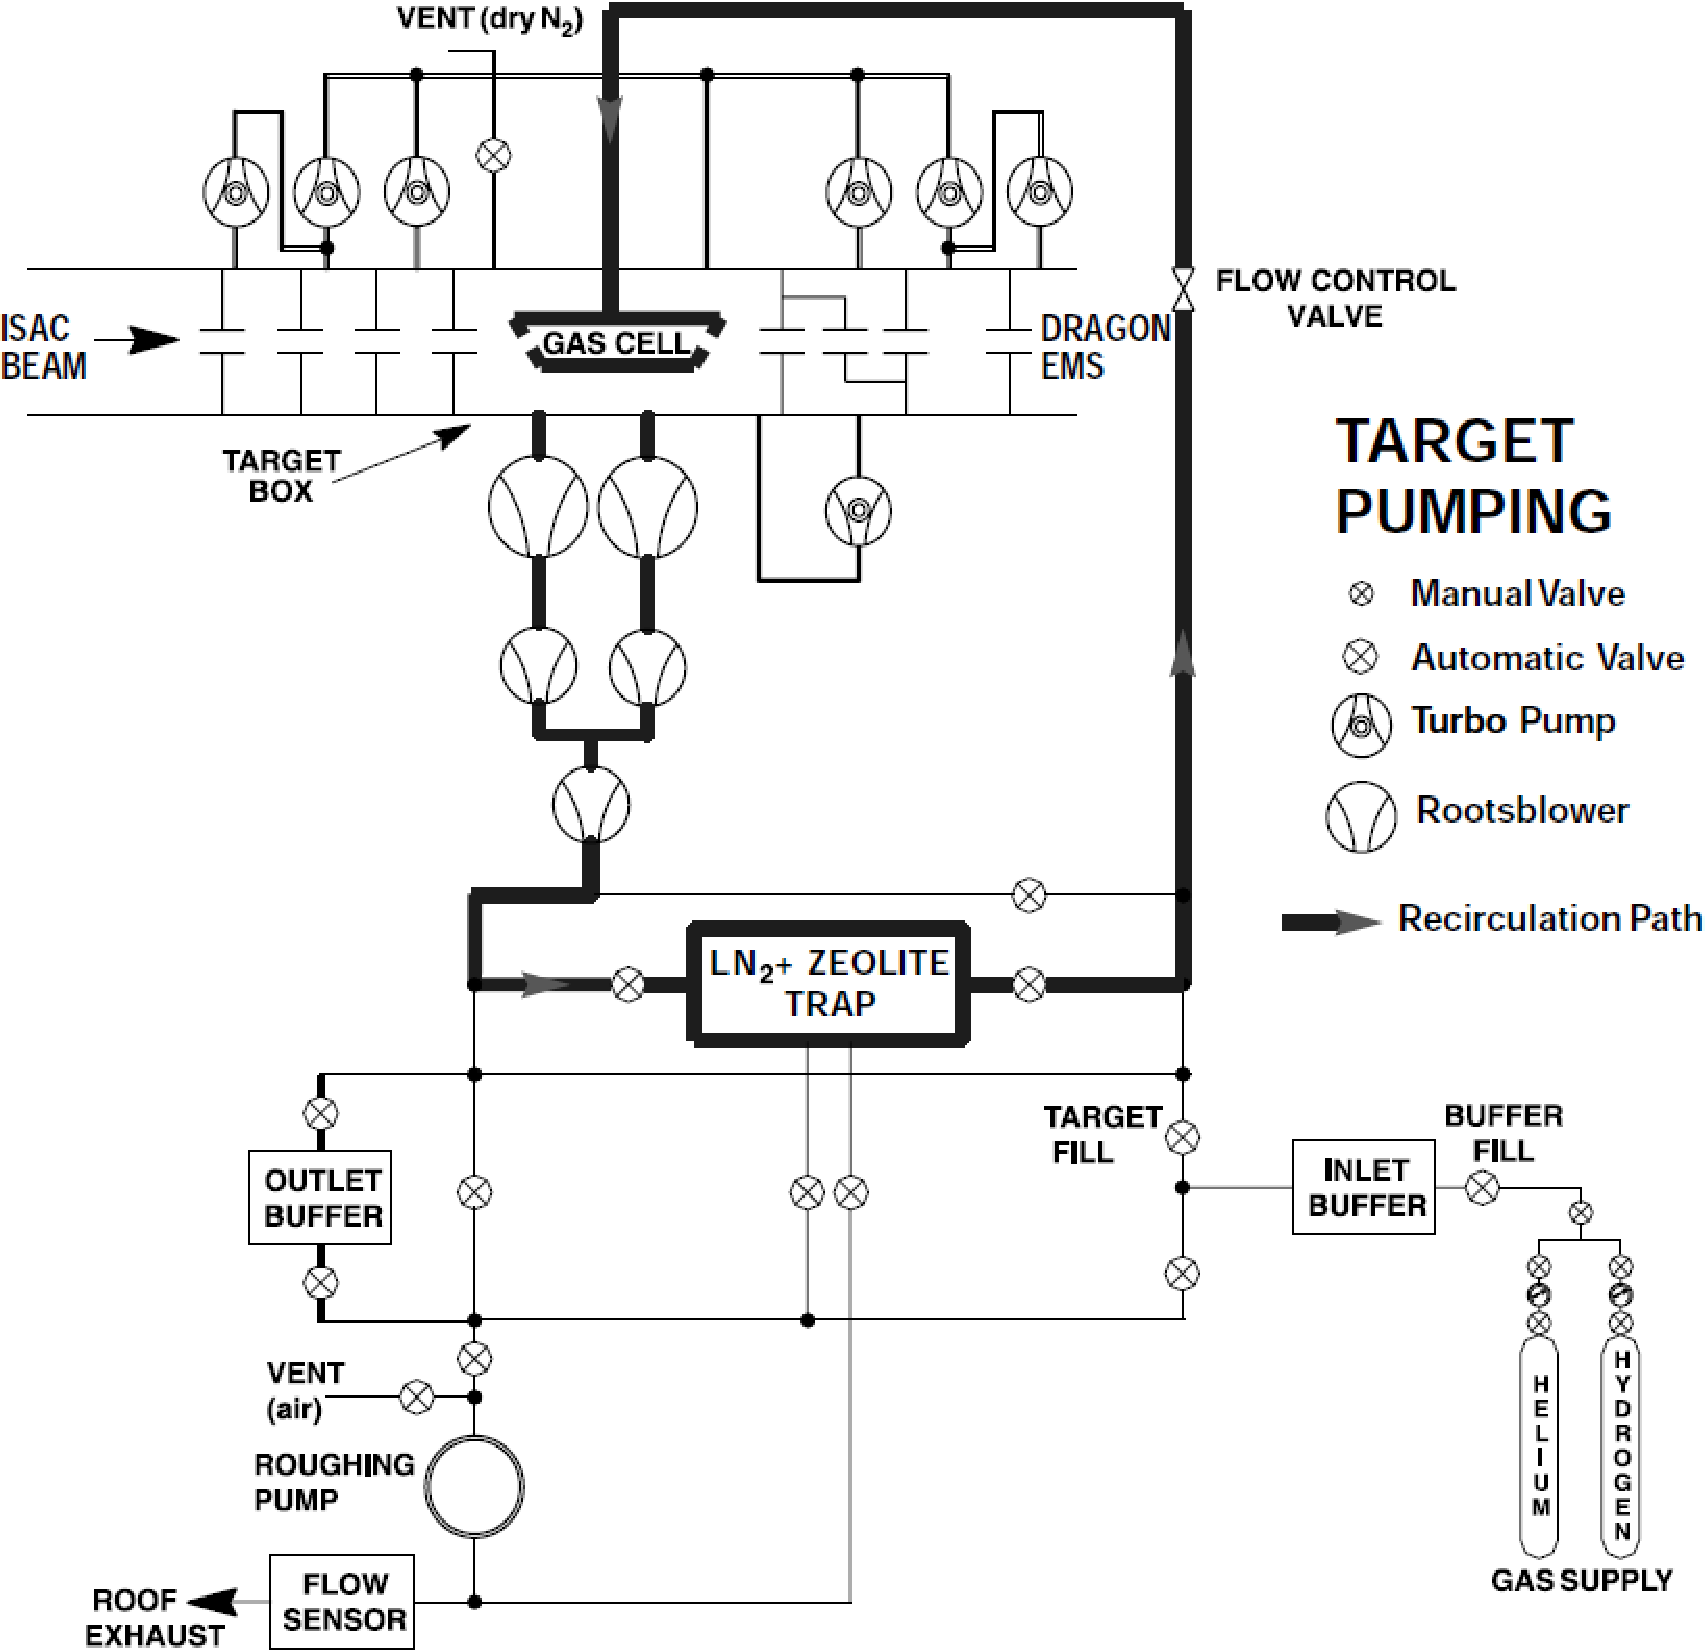
\includegraphics{Hutcheon03_Fig5_DRAGON-gastargetpumps}
}
%\vspace{5cm}       % Give the correct figure height in cm
\caption{DRAGON gas target pumping scheme. Taken from \cite{hutc03b}.}
\label{fig:dragon_pumping}
\end{figure}

%%%%%
\subsubsection{Extended length target considerations}
For the extraction of a cross section or resonance strength from the measured yield we require knowledge of the stopping power of the heavy ions in hydrogen or helium. While these are typically taken from the widely used SRIM code \cite{zieg}, recent experiments \cite{grei04} have shown deviations of the order of 20--30\% from the semi-empirical values. Therefore, direct measurement of the respective stopping power should, where possible, be preferred. This is possible when the effective length (defined as the equivalent length of constant pressure gas to achieve the same total mean ion energy loss as the non-uniform distribution) of the target is known. If the separator has full acceptance for the entire length of the target, this can be obtained through the use of a narrow-resonance reaction of known yield, otherwise it is necessary to also make measurements with small pinhole apertures. 

Additionally, angle and energy scattering of the beam and recoils on their way through the target gas needs to be estimated and taken into account in the calculation of the required recoil separator acceptance. While the ions pass through the target gas they undergo charge-changing collisions. If the target is thick enough, an equilibrium charge state distribution is achieved (semi-empirical description available in {\it e.g.} \cite{liu03}). However, if the reaction recoil originates from the downstream side of the gas target, the remaining gas track length is not sufficient to reach this equilibrium, and it is advisable to obtain the charge state distribution by tuning the recoil separator for measurements of the several charge states expected to be most abundant. For reactions where the yield is spread out over the entire length of the target, e.g. direct capture, the differing charge state distribution from the non-equilibrated recoils originating from the downstream part of the target can give rise to transmission efficiency problems. Measurements of the charge state distribution at low pressures can shed some light on this, and allow models to be set up to predict the overall detection efficiency. Some detailed consideration of charge state distributions over the length of extended targets has been done in \cite{sch04} and \cite{zyl07}, for example.

An extended target also allows the interesting possibility of determining the resonance position. It has been shown in \cite{hut12} that a the reaction $\gamma$-ray hit pattern detected in coincidence with recoils can result in a determination of the resonance position with respect to the target centre. Combining this with knowledge of the effective length and the measured stopping power, this enables a quite precise way of determining resonance energy. This can be important when yields are too low to expect measurements to be made at many closely-spaced beam energies to produce an excitation function, the usual method of resonance energy determination. 


%%%%%
\subsubsection{Gas jet targets}
Especially for the astrophysically most important reactions \nuc{12}{C}\reac{\alpha}{\gamma}\nuc{16}{O} and \nuc{15}{O}\reac{\alpha}{\gamma}\nuc{19}{Ne}, the recoil cone angles are quite demanding on separator acceptance. In order not to aggravate the problem through the use of an extended gas target length of 5 -- 10 cm, recent discussions have proposed the use of a gas jet target with approximately 4 -- 5 mm jet diameter matched to the dimension of the incoming ion beam. Recent work on such a target has begun through the {\em Jet Experiments in Nuclear Structure and Astrophysics} (JENSA) collaboration, with a view to application in future facilities such as FRIB (USA) \cite{chi13}. 

As can be seen in the pumping scheme (fig. \ref{fig:jensa}) for an appropriate gas jet target ($\approx 5\times10^{18} \unit{cm^{-2}}$ areal density), such a setup (which has been constructed and tested at Oak Ridge National Laboratory and is currently being deployed at the NSCL/ReA3 facility) requires significantly more powerful pumping stages as well as expensive gas compression and cleaning.\\
 
\begin{figure}
\resizebox{0.98\columnwidth}{!}{
\includegraphics{pumpschematic2}
}
%\vspace{5cm}       % Give the correct figure height in cm
\caption{Pumping scheme for the JENSA gas jet target. See \cite{chi13} for more details.}
\label{fig:jensa}
\end{figure}
%\small
%\begin{itemize} 
%\item What are the advantages of using a differentially pumped windowless gas target?
%\item for our purpose H and He targets best solution as he not available implanted in sufficient densities; H possibles but about factor 4 yield advantage due to 1/stopping term in resonant yeild equation
%\item also indestructible and stable in composition (plastic foils change and have current limit)
%\item windows are detrimental to recoil transmission, therefor windowless, differentially pumped approach ideal for our application
%\item what thickness to chooses: resonance width (usually small) + uncertainty in resonance position (info from transfer reactions plus knowledge of masses of reaction partners of order a few keV) follows target thickness of about 10 kev in CM system is useful leading areal target densities aspired of 5E18 1/cm2
%\item at 7-8 Torr achieved with about 10 cm length
%\item give equation from Rolfs for gas target density
%\item  length of target determines origin of recoil; needs to be matched with acceptance of the recoil separator (shorter is better); some reactions would benefit from gas jet which is however technically more challenging due to the large gas flow rates involved.
%\item Gas flow limiting apertures need to be matched to the heavy (radioactive) ion beam properties and the nuclear reaction recoil cone angle
%\item we need to know stopping powers; found differences to SRIM of the order of 20-30% when we measured ourselves
%\item energy and angle scattering needs to be estimated and included in acceptances; not well known
%\item charge state distributions, often equilibrium not achieved; preferably to be measured in experiment
%\end{itemize}
%\normalsize




